\section{Wellocate: a simulated assay campaign}
\label{sec:env}

\emph{Wellocate} turns an assay campaign into an episode with a score (Figure~\ref{fig:env}). We copy its shape
from two real protein experiments, deep mutational scans that set out to measure every variant at four positions of GB1 and of
PhoQ \citep{wu2016adaptation,podgornaia2015phoq}. A candidate is a string of four letters, one per position, from a
20-letter alphabet, one letter for each amino acid, so the space holds 160{,}000 candidates. Each candidate has a hidden
true value, its quality, which the agent never sees.

The true values come from a landscape, a fixed table that gives every candidate its value. We use three. One is
synthetic: a generated NK landscape \citep{kauffman1989nk} that we call the grid (Figure~\ref{fig:gridland}). Each of
its four positions gets a score between 0 and 1 from a fixed random table, and the score depends on that position's
letter and the next position's letter. A candidate's true value is the average of its four scores. The main study runs on the grid because every true value is known exactly and no model can
have seen its optimum. Two are real: the published landscapes of GB1 \citep{wu2016adaptation} and PhoQ \citep{podgornaia2015phoq}. We run
the same agents on them to check that what we find on the grid also holds on real biology. A model may have memorised
these, so their amino-acid names are replaced by the letters A to T through a random map at each position. Each variant keeps its
measured value under its new name, and two variants that differ by a single mutation in the real protein still
differ by a single letter after the renaming. The scrambled landscape is therefore exactly as hard to search as the real one, and a model cannot answer
from memory. Each landscape has its own best candidate (\texttt{IOJO} on the grid). We multiply every value in a
landscape by one constant so that its best candidate scores 8.762, the top reading in the GB1 data; this puts all
three on one scale and changes no ranking. The two kinds of landscape also become the two
tracks of the benchmark we release (Section~\ref{sec:bench}): the \emph{grid} track generates fresh NK landscapes, and the \emph{protein} track uses fresh scrambles of GB1 and PhoQ.

Most candidates do not work at all. In a real protein, most random variants do not fold or
lose their function, and a search has to find the few that work. We call a candidate \emph{viable} if its true value is in the top 7\%
of its landscape, and use the same 7\% on all three landscapes (Figure~\ref{fig:gridland}a). The share is close to the share of GB1 variants that keep at least a tenth of the
wild type's fitness (\nGbViable\%). The agent is not told which candidates are viable. Viable candidates cluster, so the neighbours of a working candidate are a good place to look. Take any viable candidate
and its \nNbrPer{} neighbours, the candidates one letter away (19 other letters at each of 4 positions): on the grid,
\nNbrViableGrid\% of those neighbours are viable on average, against 7\% of all candidates
(Figure~\ref{fig:gridland}b). The two real landscapes cluster more strongly (\nNbrViableGb\% on GB1,
\nNbrViablePq\% on PhoQ), so the grid does not make the search easier than real data would.

A campaign has 15 rounds of 4 slots, one slot per assay well, 60 measurements in all. Every campaign starts from the
same candidate, the median viable one (\texttt{GDIF} on the grid), and the agent is told its value, as a lab starts
from a variant it already knows. One shared start gives every model the same search. Each round the agent orders
four candidates, and the environment, which holds every true value, handles each order. It rejects an order for a
non-viable candidate before the order uses a slot and asks the agent for a replacement; if three replacements in a
row are also rejected, the slot is lost. It fails about 15\% of orders for viable candidates at random, whatever
their value: nothing comes back, and the slot is still spent. Every other order returns a reading: the candidate's
true value plus noise with a standard deviation of 7.3\% of that value. The 7.3\% is the counting error of the
GB1 deep mutational scan \citep{wu2016adaptation}: on average it read each variant's DNA about 557 times before selection and 285
times after, and counting at those depths gives a relative error of about 7.3\% (Appendix~\ref{app:noise}). The environment keeps the record of
every order, rejection, failure and reading, and shows the agent the full record before each round. The agent may
order a candidate it has already measured. At the end it nominates one candidate, scored on its true value. The budget and the failure rate are design choices: the budget is sized for slow assays in which each measurement is costly.

\begin{figure}[tbp]
\centering
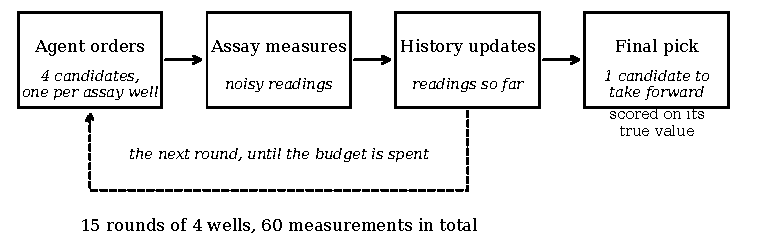
\includegraphics[width=\textwidth]{fig1_environment.pdf}
\caption{One Wellocate campaign, with the lab counterpart of each part. Each round the agent orders four candidates,
one per assay well. The simulated assay returns a noisy reading for each, and the agent sees every reading so far
before ordering again. Orders for non-viable candidates are rejected and replaced, and about 15\% of orders for viable candidates
fail. After 15 rounds the agent nominates the candidate to take forward, scored on its true value.}
\label{fig:env}
\end{figure}

Each piece of the campaign has a lab counterpart. A slot is an assay well. A failed order is a failed assay. A
non-viable candidate is a variant that does not fold or express, caught here before it uses a well. The noise is
replicate variability: the same variant measured twice gives two different numbers. The nominee is the variant taken
forward. Appendix~\ref{app:env} lists where the environment is simpler than a lab, and the direction of each
simplification.

\begin{figure}[tbp]
\centering
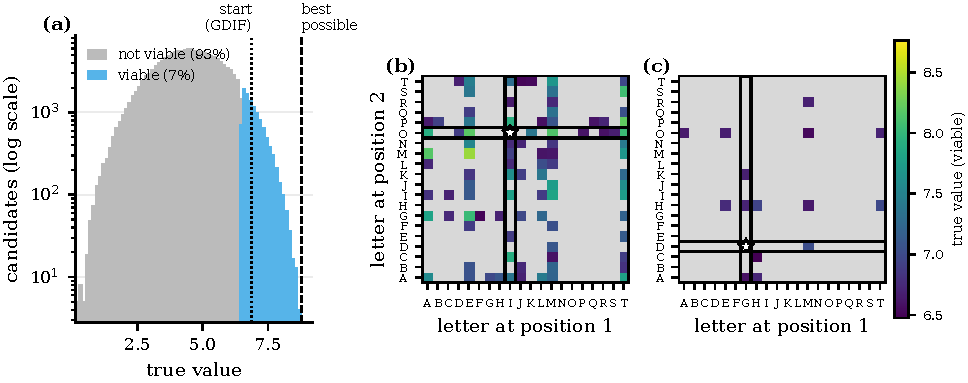
\includegraphics[width=\textwidth]{fig_landscape_env.pdf}
\caption{The grid. (a) True value of all 160{,}000 candidates. A value averages four random position scores, so
most candidates sit near the middle and very high or very low values are rare; the vertical axis is on a log scale
so that the rare ones show. Only the top 7\% (11{,}199) are viable, shown in
blue; an order for any other candidate is rejected. Every campaign starts from \texttt{GDIF}, the median viable
candidate (6.87), and the best possible is 8.762. (b, c) A candidate has four letters, so each grid shows one
slice: letters 3 and 4 are fixed and letters 1 and 2 vary, 400 candidates per slice. Grey cells are not viable.
Changing only letter 1 moves along the star's row, and changing only letter 2 moves along its column, so the
outlined row and column hold the \nSliceNbrs{} candidates one letter away that a slice can show. (b) The slice through
the best candidate, \texttt{IOJO}, with J and O fixed: \nSliceViablePct\% of the slice is viable, and
\nSliceNbrsViable{} of the star's \nSliceNbrs{} outlined neighbours. This is the richest region of the grid. (c) The
slice through the start, \texttt{GDIF}, with I and F fixed: \nStartSliceViable{} of \nStartSliceCells{} cells are
viable, and \nStartRowColViable{} of the star's \nStartRowCol{} outlined neighbours. \nStartOffSliceViable{} of the
start's \nStartNbrsGrid{} viable neighbours change letter 3 or 4 and so lie off this slice. The search problem is
getting from (c) to (b).}
\label{fig:gridland}
\end{figure}

A finished campaign leaves two things to score: how the agent spent its slots, and how good its final pick was. To score how the slots were spent, we use the \emph{re-testing share}, the fraction of used slots spent on a candidate the agent had already ordered. An agent that orders the same candidate in all four slots of a round re-tests three of them.
The share counts repeats over the whole campaign, whichever candidates they went to; how many readings lie behind
the final pick is a separate count, reported in Section~\ref{sec:both}. To score the final pick, we split
the final pick's shortfall from the best candidate in the landscape into two parts that add up, both computed from
true values, which the agent never sees. The \emph{exploration loss} is how far the best candidate the agent measured
falls short of the landscape's best; it is large when the search never reached the good candidates. The
\emph{selection loss} is how far the nominated candidate falls short of the best candidate the agent measured; it is large when the agent found a good candidate and then nominated a worse one. Selection loss comes from noise: the agent can rank
candidates only by their readings, and a candidate measured once can read well above its true value and look better
than one that is truly better. Re-testing averages this noise away and shrinks the selection loss. Each re-test also takes a slot from a new candidate, which can raise the exploration loss.

A re-testing share on its own does not say whether an agent re-tests too much or too little, so we need a yardstick.
We use three simple fixed strategies, together called the \emph{scripted rules}: the guessing rule, the informed
rule and the model-guided rule. All three work under the same budget, noise and order format as the agents. Each round, the \emph{guessing rule} re-tests its current best a fixed number of times and fills the other slots
with untried neighbours of it, candidates one letter away, guessing which ones are viable, as the agents must. The \emph{informed rule} does the same and is also told which candidates are viable, so it is never rejected; it still has to measure how good they are. For these two rules we set the number of re-tests per round after the runs, to the one with the
best mean true pick on each landscape, a tuning the agents do not get. The \emph{model-guided rule} learns from its own
readings only. It scores each letter at each position by the mean reading of the measured candidates that carry it,
and adds these scores to rank untried one- and two-letter changes of its current best. It re-tests one leading
candidate each round and spends its last three rounds re-testing its four best. Appendix~\ref{app:refs} gives the
settings of all three.

Against this yardstick we run five language models: Opus 4.7, Gemini 2.5 Flash, DeepSeek V3.1, GPT-6.1 Sol and
Gemini 3.1 Pro, each as a minimal agent. Every round it receives one prompt holding the task and the full history of its orders and readings, and it replies with its orders. That history, written by the environment, is its only memory of earlier rounds:
the model itself carries nothing from one call to the next, and it has no tools or scaffold. We chose this on purpose, so that what we measure is the model's own allocation. 
